\input{../tex/preambule}
\usepackage{tikz}
\usepackage{inputenc}
\usetikzlibrary{arrows,automata}
\usetikzlibrary{positioning}
\geometry{top=3cm,bottom=3cm}

\title{\vspace{\fill}\textbf{\Huge Organigramme}}
\author{Sonny Klotz - Jean-Didier Pailleux - Malek Zemni\vspace{2em}\\\textit{Interface de chargement, de contrôle}\\\textit{et d’analyse statistique des données}\\\textit{pour la constitution d’un graphe de flux}\vspace{2em}}

\begin{document}
\maketitle\vspace{\fill}
\newpage
	
	\section{Présentation de l'organigramme}
		Le travail peut être décomposé en 3 modules :
		\begin{itemize}
		\item Une interface graphique : va faire transiter les informations entre les différentes APIs de l'application et fournir des rendus visuels des analyses
		\item Une API de chargement des données : va effectuer des vérifications sur les données fournies (\lstinline!.csv!) puis retourne le résultat à l'interface graphique
		\item Une API d'analyse descriptive des données : va permettre de calculer les informations statistiques nécessaires
		\end{itemize}
		
		\begin{center}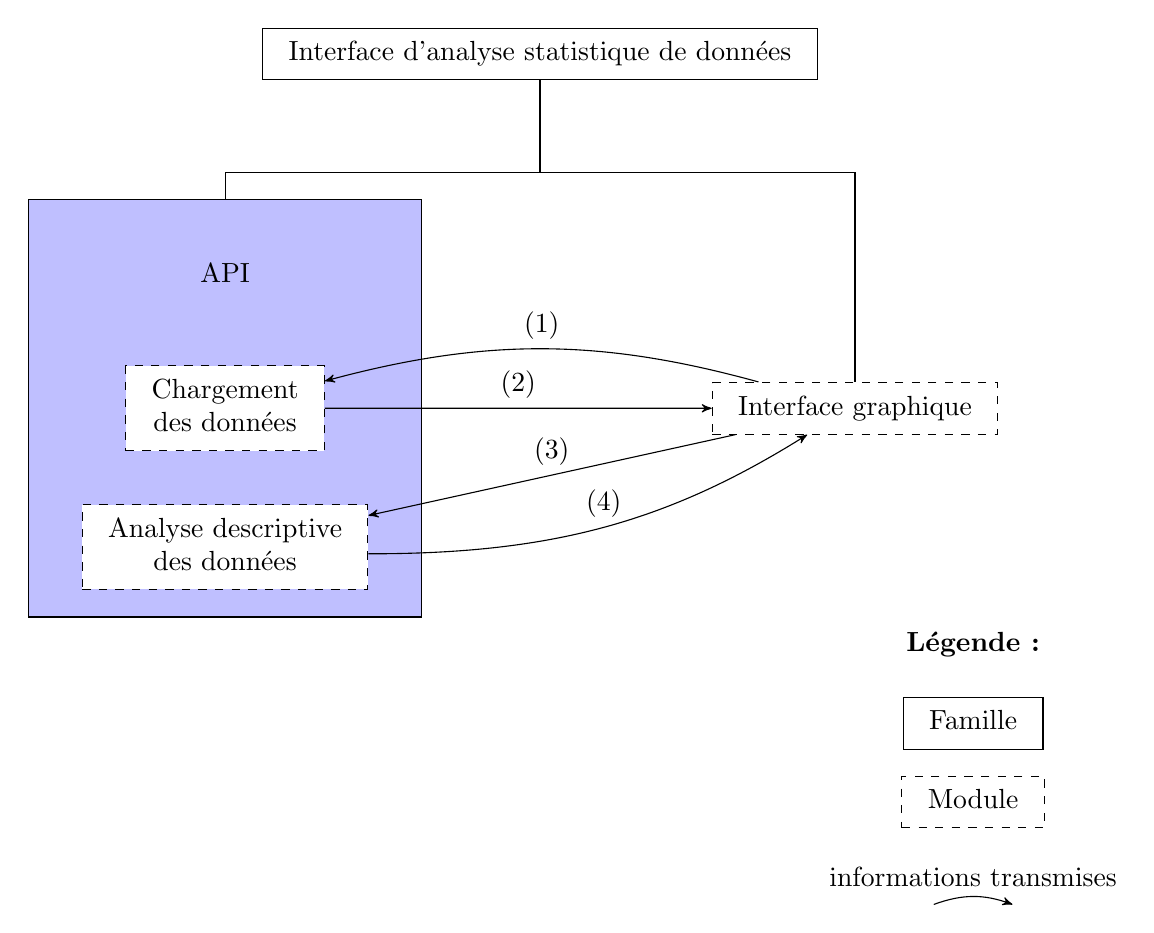
\begin{tikzpicture}
			\begin{scope}[xscale=2,yscale=1.5]	
				% description et nommage des noeuds 
				\node (TITRE) at (0,7) [rectangle,draw] {\begin{tabular}{c}Interface d'analyse statistique de données\end{tabular}};
				\node (API) at (-2,4) [rectangle,draw,fill=blue!25,text depth=3.5cm,minimum width=5cm,minimum height=5.3cm,font=\textbf\Large] {\begin{tabular}{c}API\end{tabular}};
				\node (CHRG) [rectangle,draw,dashed,fill=white] at (API.center){\begin{tabular}{c}Chargement\\des données\end{tabular}};
				\node (ADD) [rectangle,draw,dashed,fill=white] at ([yshift=1.7em]API.south){\begin{tabular}{c}Analyse descriptive\\des données\end{tabular}};	
				\node (IG) at (2,4) [rectangle,draw,dashed] {\begin{tabular}{c}Interface graphique\end{tabular}};
				% description des arêtes
				% -- arête rectiligne entre les noeuds nommés ou indiqués en coordonnées
				% |- départ vertical arrivée horizontale
				% -| départ horizontal arrivée verticale
				\draw (TITRE) |- (-2,6);
				\draw (TITRE) |- (2,6);
				\draw (-2,6) -- (API);
				\draw (2,6) -- (IG);
				\path[->,>=stealth'] (IG) edge[bend left=-20] node[anchor=south,above]{(1)} (CHRG);
				\path[->,>=stealth'] (CHRG) edge[bend left=0] node[anchor=south,above]{(2)} (IG);
				\path[->,>=stealth'] (IG) edge[bend left=0] node[anchor=south,above]{(3)} (ADD);
				\path[->,>=stealth'] (ADD) edge[bend left=-20] node[anchor=south,above]{(4)} (IG);
			\end{scope}
			%Légende
			\begin{scope}
				\node (LEGENDE) at (5.5,3) {\textbf{Légende :}};
				\node (FAMILLE) at (5.5,2) [rectangle,draw] {\begin{tabular}{c}Famille\end{tabular}};
				\node (MODULE) at (5.5,1) [rectangle,draw,dashed] {\begin{tabular}{c}Module\end{tabular}};
				\path[->,>=stealth'] (5,-0.3) edge[bend left=20] node[anchor=south,above]{informations transmises} (6,-0.3);
			\end{scope}
		\end{tikzpicture}\end{center}
		
		\begin{center}\begin{figure}[h]
			\textbf{Notes :}\\
			(1) Fichier \lstinline!.csv! formaté \\
			(2) Structure décrivant les données du fichier \lstinline!.csv! après vérification : nombre de lignes et de colonnes, entrées erronées, noms des colonnes...\\
			(3) Colonne de données d'un type attendu\\
			(4) Résultats statistiques (moyenne, quantiles, ecart-type, ...)
			\caption{Organigramme des différents modules du logiciel}\label{fig:M1}
		\end{figure}\end{center}
	
	\section{Fonctionnalités des modules}
		\subsection{API}
			\textit{Application Programming Interface} constituent les paquets utilisables par les développeurs (intégrée), qu'on va livrer au client en plus de l'application elle-même.\\
			Parmi les modules du logiciel, on a 2 APIs :
			\begin{itemize}
				\item Une API de chargement des données
				\item Une API d'analyse statistique des données
			\end{itemize}
		
			\subsubsection{Chargement des données}
				Le module de chargement des données s'occupe de la préparation et de la vérification du fichier fourni en entrée. Ces principales fonctionnalités sont :
				\begin{itemize}
				\item Ouverture du fichier en vérifiant qu'il a la bonne extension \lstinline!.csv! et qu'il est accessible en lecture.
				\item Donner le nombre de lignes et de colonnes
				\item Détection des type de colonnes : ça sera plutôt une détection de la cohérence des types, on parcourt les entrées de chaque colonne et on vérifie si leur type correspond bien au type attendu.\\
				Dans le même parcours, on pourra aussi gérer les erreurs :
					\begin{itemize}
					\item détecter les valeurs erronées (valeurs qui ne correspondent pas au type attendu)
					\item détecter les cases vides
					\end{itemize}
				\item Nommer les colonnes.
				\end{itemize}
				En sortie, on aura donc une structure décrivant les données du fichier \lstinline!.csv! après vérification : nombre de lignes et de colonnes, entrées erronées, noms des colonnes...
				
			\subsubsection{Analyse descriptive des données}
				Ce module est utilisé pour fournir des informations de statistiques descriptives sur les colonnes de données qui lui seront fournies. Ses fonctionnalités se décomposent en trois pour les différents types de données à traiter:\\
				\begin{enumerate}
				\item qualitatif : calcul des effctifs et fréquences d'apparition
				\item quantitatif discret :\\
					\begin{itemize}
					\item effectifs, effectifs cumulés, fréquence et fréquence cumulée
					\item moyenne
					\item médiane et autres quantiles
					\item variance et écart-type
					\item anomalies : boîte à moutaches de Tukey
					\item symétrie : coeff de Pearson ou coeff de Yule
					\item aplatissement : coeff de Fisher
					\end{itemize}
				\item quantitatif continu : on regroupe les valeurs en classe d'intervalles, on peut ensuite appliquer les mêmes techniques que pour les variables discrètes
				\end{enumerate}
			
		\subsection{Interface graphique}
			Le module de l'interface graphique s'occupera de la manière dont l'application sera représentée à l'écran pour l'utilisateur, ce qui correspond au positionnement des éléments textuels, boutons et des fonctionnalités disponible dans une fenêtre. Voici une liste des principales fenêtres composant ce module avec leurs fonctionnalités:
			\begin{enumerate}
			\item Fenêtre de chargement pour récupérer un fichier \lstinline!.csv! avec validation du choix pour passer à la prochaine fenêtre (En renseignant son chemin dans le système de fichier, ou de la manière d'un Drag \& Drop).
			\item Fenêtre de contrôle préliminaire avec visualisation d'un échantillon du \lstinline!.csv!.		
				\begin{itemize}
				\item Affichera le nombre de lignes/colonnes contenu dans le .csv.
				\item Affichera le titre du fichier.
				\item Affichera un échantillon du contenu du \lstinline!.csv! (environ les 1000 premières lignes) avec un système de scroll.
				\item Affichage des lignes erronés (numéro de la ligne + contenu + type d'erreur).
				\item Mise en place d'un système de navigation sous forme d'onglet (Onglet erreurs, onglet échantillon,...). Cela permettra d'éviter que la fenêtre contienne trop d'informations.
				\item Affichage d'un bouton pour passer à l'étape de l'analyse de données.
				\end{itemize}
			\item Fenêtre correspondant à l'étape de l'analyse de données.
				\begin{itemize}
				\item L'Utilisateur devra sélectionner la colonne avec un clic, puis pourra lancer l'analyse sur celle-ci.
				\item La fenêtre affichera les résultats de l'étude qualitative (Médiane, Quantile et anomalie) d'une part et de l'étude quantitative (Histogramme et Diagramme de secteur) d'autre part.
				\item Un bouton pour lancer l'exportation des résultats sera disponible (Écriture dans un nouveau fichiers).
				\end{itemize}
			\end{enumerate}
		
		
	
\end{document}
